%%%%%%%%%%%%%%%%%%%%%%%%%%%%%%%%%%%%%%%%%
% Lachaise Assignment
% LaTeX Template
% Version 1.0 (26/6/2018)
%
% This template originates from: http://www.LaTeXTemplates.com
%
% Authors:
% Marion Lachaise & François Févotte
% Vel (vel@LaTeXTemplates.com)
%
% License:
% CC BY-NC-SA 3.0 (http://creativecommons.org/licenses/by-nc-sa/3.0/)
%
%%%%%%%%%%%%%%%%%%%%%%%%%%%%%%%%%%%%%%%%%

%----------------------------------------------------------------------------------------
%	PACKAGES AND OTHER DOCUMENT CONFIGURATIONS
%---------------------------------------------------------------------------------------- 
\documentclass{article}

%%%%%%%%%%%%%%%%%%%%%%%%%%%%%%%%%%%%%%%%%
% Lachaise Assignment
% Structure Specification File
% Version 1.0 (26/6/2018)
%
% This template originates from:
% http://www.LaTeXTemplates.com
%
% Authors:
% Marion Lachaise & François Févotte
% Vel (vel@LaTeXTemplates.com)
%
% License:
% CC BY-NC-SA 3.0 (http://creativecommons.org/licenses/by-nc-sa/3.0/)
%
%%%%%%%%%%%%%%%%%%%%%%%%%%%%%%%%%%%%%%%%%

%----------------------------------------------------------------------------------------
%	!!!CUSTOM!!!
%----------------------------------------------------------------------------------------

\usepackage[english]{babel}
\usepackage[ngerman]{datetime}

\newdateformat{myformat}{\THEDAY{.  }\monthnamengerman[\THEMONTH], \THEYEAR}

\usepackage{xcolor}

%----------------------------------------------------------------------------------------
%	PACKAGES AND OTHER DOCUMENT CONFIGURATIONS
%----------------------------------------------------------------------------------------

% TODO changed
% \usepackage{amsmath,amsfonts,stmaryrd,amssymb} % Math packages
\usepackage{amsmath,amsfonts,amssymb} % Math packages

\usepackage{enumerate} % Custom item numbers for enumerations

% TODO
% \usepackage[ruled]{algorithm2e} % Algorithms

\usepackage[framemethod=tikz]{mdframed} % Allows defining custom boxed/framed environments

\usepackage{listings} % File listings, with syntax highlighting
\lstset{
	basicstyle=\ttfamily, % Typeset listings in monospace font
}

%----------------------------------------------------------------------------------------
%	DOCUMENT MARGINS
%----------------------------------------------------------------------------------------

\usepackage{geometry} % Required for adjusting page dimensions and margins

\geometry{
	paper=a4paper, % Paper size, change to letterpaper for US letter size
	top=2.5cm, % Top margin
	bottom=3cm, % Bottom margin
	left=2.5cm, % Left margin
	right=2.5cm, % Right margin
	headheight=14pt, % Header height
	footskip=1.5cm, % Space from the bottom margin to the baseline of the footer
	headsep=1.2cm, % Space from the top margin to the baseline of the header
	%showframe, % Uncomment to show how the type block is set on the page
}

%----------------------------------------------------------------------------------------
%	FONTS
%----------------------------------------------------------------------------------------

\usepackage[utf8]{inputenc} % Required for inputting international characters
\usepackage[T1]{fontenc} % Output font encoding for international characters

\usepackage{XCharter} % Use the XCharter fonts

%----------------------------------------------------------------------------------------
%	COMMAND LINE ENVIRONMENT
%----------------------------------------------------------------------------------------

% Usage:
% \begin{commandline}
%	\begin{verbatim}
%		$ ls
%		
%		Applications	Desktop	...
%	\end{verbatim}
% \end{commandline}

\mdfdefinestyle{commandline}{
	leftmargin=10pt,
	rightmargin=10pt,
	innerleftmargin=15pt,
	middlelinecolor=black!50!white,
	middlelinewidth=2pt,
	frametitlerule=false,
	backgroundcolor=black!5!white,
	frametitle={Command Line},
	frametitlefont={\normalfont\sffamily\color{white}\hspace{-1em}},
	frametitlebackgroundcolor=black!50!white,
	nobreak,
}

% Define a custom environment for command-line snapshots
\newenvironment{commandline}{
	\medskip
	\begin{mdframed}[style=commandline]
}{
	\end{mdframed}
	\medskip
}

%----------------------------------------------------------------------------------------
%	FILE CONTENTS ENVIRONMENT
%----------------------------------------------------------------------------------------

% Usage:
% \begin{file}[optional filename, defaults to "File"]
%	File contents, for example, with a listings environment
% \end{file}

\mdfdefinestyle{file}{
	innertopmargin=1.6\baselineskip,
	innerbottommargin=0.8\baselineskip,
	topline=false, bottomline=false,
	leftline=false, rightline=false,
	leftmargin=2cm,
	rightmargin=2cm,
	singleextra={%
		\draw[fill=black!10!white](P)++(0,-1.2em)rectangle(P-|O);
		\node[anchor=north west]
		at(P-|O){\ttfamily\mdfilename};
		%
		\def\l{3em}
		\draw(O-|P)++(-\l,0)--++(\l,\l)--(P)--(P-|O)--(O)--cycle;
		\draw(O-|P)++(-\l,0)--++(0,\l)--++(\l,0);
	},
	nobreak,
}

% Define a custom environment for file contents
\newenvironment{file}[1][File]{ % Set the default filename to "File"
	\medskip
	\newcommand{\mdfilename}{#1}
	\begin{mdframed}[style=file]
}{
	\end{mdframed}
	\medskip
}

%----------------------------------------------------------------------------------------
%	NUMBERED QUESTIONS ENVIRONMENT
%----------------------------------------------------------------------------------------

% Usage:
% \begin{question}[optional title]
%	Question contents
% \end{question}

\mdfdefinestyle{question}{
	innertopmargin=1.2\baselineskip,
	innerbottommargin=0.8\baselineskip,
	roundcorner=5pt,
	nobreak,
	singleextra={%
		\draw(P-|O)node[xshift=1em,anchor=west,fill=white,draw,rounded corners=5pt]{%
		Question \theQuestion\questionTitle};
	},
}

\newcounter{Question} % Stores the current question number that gets iterated with each new question

% Define a custom environment for numbered questions
\newenvironment{question}[1][\unskip]{
	\bigskip
	\stepcounter{Question}
	\newcommand{\questionTitle}{~#1}
	\begin{mdframed}[style=question]
}{
	\end{mdframed}
	\medskip
}

%----------------------------------------------------------------------------------------
%	WARNING TEXT ENVIRONMENT
%----------------------------------------------------------------------------------------

% Usage:
% \begin{warn}[optional title, defaults to "Warning:"]
%	Contents
% \end{warn}

\mdfdefinestyle{warning}{
	topline=false, bottomline=false,
	leftline=false, rightline=false,
	nobreak,
	singleextra={%
		\draw(P-|O)++(-0.5em,0)node(tmp1){};
		\draw(P-|O)++(0.5em,0)node(tmp2){};
		\fill[black,rotate around={45:(P-|O)}](tmp1)rectangle(tmp2);
		\node at(P-|O){\color{white}\scriptsize\bf !};
		\draw[very thick](P-|O)++(0,-1em)--(O);%--(O-|P);
	}
}

% Define a custom environment for warning text
\newenvironment{warn}[1][Warning:]{ % Set the default warning to "Warning:"
	\medskip
	\begin{mdframed}[style=warning]
		\noindent{\textbf{#1}}
}{
	\end{mdframed}
}

%----------------------------------------------------------------------------------------
%	INFORMATION ENVIRONMENT
%----------------------------------------------------------------------------------------

% Usage:
% \begin{info}[optional title, defaults to "Info:"]
% 	contents
% 	\end{info}

\mdfdefinestyle{info}{%
	topline=false, bottomline=false,
	leftline=false, rightline=false,
	nobreak,
	singleextra={%
		\fill[black](P-|O)circle[radius=0.4em];
		\node at(P-|O){\color{white}\scriptsize\bf i};
		\draw[very thick](P-|O)++(0,-0.8em)--(O);%--(O-|P);
	}
}

% Define a custom environment for information
\newenvironment{info}[1][Info:]{ % Set the default title to "Info:"
	\medskip
	\begin{mdframed}[style=info]
		\noindent{\textbf{#1}}
}{
	\end{mdframed}
}
 % Include the file specifying the document structure and custom commands


%----------------------------------------------------------------------------------------
%	ASSIGNMENT INFORMATION
%----------------------------------------------------------------------------------------

\title{Huffman Code} % Title of the assignment

\date{Albert-Einstein-Schule Ettlingen --- \myformat\today} % University, school and/or department name(s) and a date


%----------------------------------------------------------------------------------------

\begin{document}

\maketitle % Print the title

%----------------------------------------------------------------------------------------
%	INTRODUCTION
%----------------------------------------------------------------------------------------

\section{Einleitung} % Unnumbered section

Um Daten zu komprimieren, kann der Huffman Code genutzt werden. Die Huffman Codierung macht sich die Tatsache zunutze, dass Buchstaben unterschiedlich oft in Texten vorkommen.
Die Länge der codierten Wörter im Huffman Code hängt dabei mit dessen Informationsgehalt zusammen. Der Huffman Code benutzt dabei einen binären Baum und wird von den Blättern zur Wurzel kodiert.
Der Huffman Code ist dabei präfixfrei. Dies hei{\ss}t, dass die Codewörter keine Trennung brauchen.

\section{Algorithmus}\cite{noauthor_<person>huffman</person>-code_nodate}

\subsection{Codierung}
Bevor man den Huffman Code codieren kann, muss erst mal ein Zeichensatz C festgelegt werden.
Jedem Zeichen c $\in$ C wird eine bestimmte Häufigkeit f(c) zugewiesen.
Daraus ergibt sich eine Prioritätenkette Q.\\

{ \color{green} Hier ein Beispiel mit dem Wort MISSISSIPPI

  $\Rightarrow$ C = \{ M,I,S,P \}
  mit Häufigkeit ergibt sich Q:
  \begin {tabular}{c c c c}
    M & P & I & S\\
    \hline
    1 & 2 & 4 & 4
  \end{tabular}
}

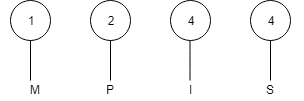
\includegraphics{./img/huffman1.png} \\
Jetzt werden die beiden Zeichen c mit der geringsten Häufigkeit f(c) mit einer Astgabelung zusammengeführt. Die beiden Häufigkeiten werden addiert und in die Astgabelung geschrieben.

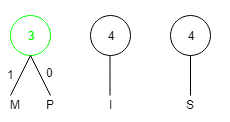
\includegraphics{./img/huffman2.png}\\

\pagebreak

Dieses Vorgehen wird fortgesetzt und es werden wieder die beiden Äste mit den geringsten Häufigkeiten zusammengeführt. Die Astgabelung wird dabei behandelt wie ein Einzelnes Zeichen.

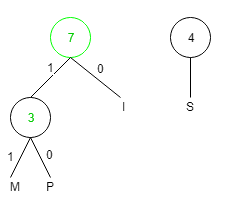
\includegraphics{./img/huffman3.png}\\

Es muss immer darauf geachtet werden die Zahlen in den Astgabelungen geordnet zu halten. Deshalb wird die Prioritätenkette neu geordnet.

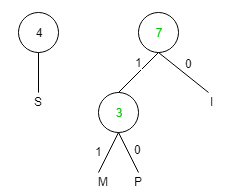
\includegraphics{./img/huffman4.png}\\
Nach der Neuordnung können wieder die beiden kleinsten Äste zusammengeführt werden und der Huffmanbaum ist fertig.

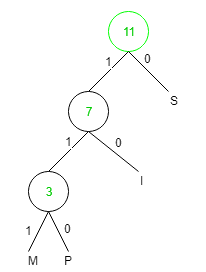
\includegraphics{./img/huffman5.png}\\
Jetzt kann aus dem Huffmanbaum die Codierung für jedes Zeichen abgelesen werden.\\

\begin {tabular}{c c c c}
    S & I & P & M\\
    \hline
    0 & 10 & 110 & 111
\end{tabular}

\section{Decodierung}

Die Decodierung des Huffman Codes ist sehr einfach, da es sich beim Huffman Code um einen präfixfreien Code handelt. Das bedeutet man benötigt keine Trennung in der Codierung zwischen den Zeichen. Bei der Decodierung folgt man dem Baum von oben nach unten bis man das Zeichen hat.

\section{Anwendungsfälle}\cite{noauthor_jpeg-kompression_nodate}

Der Huffman Code wird in zahlreichen Bereichen zur Komprimierung von Daten genutzt.
Dies ist beispielsweise bei verlustbehafteter Kompression, wie bei JPEG der Fall. Dabei wird weniger wert auf Bildqualität, sondern mehr darauf die Dateigrö{\ss}e gering zu halten.
Ein Beispiel hierfür ist das Internet. Dort ist es aufgrund der Übertragungsgeschwindigkeiten des Netzwerks von Vorteil die Bilddaten zu reduzieren, was geringere Ladezeiten als Folge hat.

\section{Optimalität}\cite{noauthor_huffman-kodierung_2019}

Beim Anwenden des Huffman Codes, wird jeder Buchstabe oder Zeichen durch einen spezifischen Code ersetzt.
Ein optimaler Code, würde dabei die Codewortlänge mindestens um die durchschnittliche Codewortlänge minimieren.
Mathematisch kann man die mittlere Codewortlänge durch eine Summe beschreiben:

\begin{enumerate}
    \item $L$ : Mittlere Codewortlänge
    \item $s_i$ : Das Ausgangssymbol
    \item $l_i$ : Länge von $s_i$
    \item $p_i$: Wahrscheinlichkeit für Ausgangssymbol oder Wort
\end{enumerate}

\[
L = \sum_{i=1}^{n} p_i * l_i
.\]\\

Ein wichtiges Merkmal beim Huffman Code ist, dass häufiger vorkommende Wörter($p_i$ ist dabei grö{\ss}er) kürzere Codes haben.
Durch den Huffman Algorithmus gilt dann für: $s_1, s_2, s_3, \ldots, s_n$:

\begin{itemize}
    \item $p_1 \ge  p_2 \ge  p_3 \ge  \ldots \ge  p_n$
    \item $l_1 \le  l_2 \le \le  l_3 \le  \ldots \le  l_n$
\end{itemize}

$\Rightarrow$ Die durch den Huffman Algorithmus vorgelegte aufsteigende Sortierung macht den Code optimal.

\section{Verbesserungen}\cite{noauthor_explain_nodate}

Trotzt dessen, dass der Huffman Code eine gute Kompression bietet, ist diese nicht optimal.
Dies ist zum Beispiel der Fall, wenn die Anzahl der häufigsten Buchstaben $P_{max}$ sehr hoch ist.

\subsection{Beispiel}

Man nehme ein Text mit den Zeichen $A = {a_1, a_2, a_3}$ und die Wahrscheinlichkeiten: $P(a_1) = 0.8, P(a_2) = 0.02 \quad \& \quad P(a_3) = 0.18$.
Die dazugehörige Huffman Codierung würde Folgenderma{\ss}en aussehen:

\begin{table}[htpb]
    \centering
    \begin{tabular}{|c c|} 
        \hline
        Zeichen & Code \\
        \hline\hline
        $a_1$ & 0\\
        \hline
        $a_2$ & 11\\
        \hline
        $a_3$ & 10\\
        \hline
    \end{tabular}
\end{table}

Die durchschnittliche Codelänge beträgt dabei:

\[
    L(C)= (\sum_{i=1}^{3}) /3 = 1,2 \frac{bits}{symbol}
.\]

Die Entropie\cite{noauthor_entropie_2019} oder der Informationsgehalt für den Text $A$ beträgt dabei:

\[
    H(X) = -\sum_{i=1}^{3} p_i * \log_2(p_i) = 0,82 \frac{bits}{symbol}
.\]

Die Redundanz für diesen Code(Differenz von $L(C)$ und $H(X)$) wäre dann:

\[
    L(C) - H(X) = 1,2 - 0,82 = 0,384 \frac{bits}{symbol}
.\]\\
Wenn man das Ergebnis mit dem eigentlichen Informationsgehalt vergleicht, kann man erkennen
dass der Code $47\%$ mehr Bits verbraucht als eigentlich nötig.

\subsubsection{Erweiterter Huffman Code}

Um die Redundanz im Huffman Code zu reduzieren, kann man anstatt ein Codewort für jedes Zeichen, ein Codewort für jeweils zwei Zeichen erstellen:

\begin{table}[htpb]
    \centering
    \begin{tabular}{|c c c|} 
        \hline
        Zeichen & Wahrscheinlichkeit & Code\\
        \hline\hline
        $a_1a_1$ & 0,64 & 0\\
        \hline\hline
        $a_1a_2$ & 0,016 & 10101\\
        \hline\hline
        $a_1a_3$ & 0,144 & 11\\
        \hline\hline
        $a_2a_1$ & 0,016 & 10100\\
        \hline\hline
        $a_2a_2$ & 0,0004 & 10100101\\
        \hline\hline
        $a_2a_3$ & 0,0036 & 10010011\\
        \hline\hline
        $a_3a_1$ & 0,1440 & 100\\
        \hline\hline
        $a_3a_2$ & 0,0036 & 10100100\\
        \hline\hline
        $a_3a_3$ & 0,0324 & 10100\\
        \hline
    \end{tabular}
\end{table}

\begin{enumerate}
    \item $L(C)_1 = 1,7228 \frac{bits}{symbol} $
    \item $L(C) = \frac{L(C)_1}{2} =  \frac{1,7228}{2} = 0,8614$
\end{enumerate}\bigskip

Da ein Symbol im erweiterten Huffman Code zwei Zeichen entspricht, ist die durchschnittliche Wortlänge kürzer.
Dies hat wiederum eine kleinere Redundanz zu Folge die nur bei $0,045 \frac{bits}{Symbol}$ liegt.
Das wären nur $5,5 \%$ des Informationsgehaltes und deshalb viel Redundanzfreier als der klassische Huffman Code.

\renewcommand{\refname}{Literaturverzeichnis}
\bibliographystyle{abbrv}
\bibliography{sources}

\end{document}
